\section{Our QA Testbed: \qb{}}\label{sec:dataset}

The ``gold standard'' of academic competitions between universities
and high schools is \qb{}. Unlike \abr{qa} formats such as
Jeopardy!~\cite{ferruci-10}, \qb{} questions are
designed to be interrupted: questions are read to two competing teams
and whoever knows the answer first interrupts the question and
``buzzes in''.

This style of play requires questions to be structured
``pyramidally''~\cite{jose2017craft}: questions start with difficult clues and get
progressively easier. These
questions are carefully crafted to
allow the most knowledgeable player to answer first. A question on
Paris that begins ``this capital of France'' would test 
reaction speed, not knowledge; thus, skilled authors arrange
the clues so players will recognize them with increasing
probability (Figure~\ref{fig:ex}).

The answers to \qb{} questions are typically well-known entities.  In
the \abr{qa} community~\cite{hirschman-01}, this is called ``factoid''
\abr{qa}: the entities come from a relatively
closed set of possible answers.

\begin{figure}[t!]
\centering
\tikz\node[draw=white!40!black,inner sep=1pt,line width=0.3mm,rounded corners=0.1cm]{
  \begin{tabular}{p{0.46\textwidth}}
    \small
The protagonist of this opera describes the future day when her lover will
arrive on a boat in the aria ``Un Bel Di'' or ``One Beautiful Day''. The only
baritone role in this opera is the consul Sharpless who reads letters for the
protagonist, who has a maid named Suzuki. That protagonist blindfolds her child
Sorrow before stabbing herself when her lover B.\ F.\ Pinkerton returns with a
wife. For 10 points, name this Gia4o Puccini opera about an American
lieutenant's affair with the Japanese woman Cio-Cio San.\\
\textbf{Answer}: \underline{Madama Butterfly}
\end{tabular}
};
\caption{An example \qb{} question. The question becomes progressively
  easier (for humans) to answer later on; thus, more knowledgeable
  players can answer after hearing fewer clues.  Our adversarial
  writing process ensures that the clues also
  challenge computers.}
   \label{fig:ex}
\end{figure}

\subsection{Known Exploits of \qb{} Questions}
\label{subsec:exploits}

Like most \abr{qa} datasets, \qb{} questions are
written for \emph{humans}. Unfortunately, the heuristics that
question authors use to select clues do not always apply to
computers. For example, humans are unlikely to memorize every song in
every opera by a particular composer. This, however, is trivial for a
computer. In particular, a simple \abr{qa} system easily
solves the example in Figure~\ref{fig:ex} from seeing the reference to
``Un Bel Di''. Other questions contain uniquely identifying ``trigger
words''~\cite{harris2006prisoner}. For example, ``martensite'' only appears in questions on
\underline{steel}. For these examples, a \abr{qa} system needs
to understand no additional information other than an if--then rule.

One might wonder if this means that factoid \abr{qa} is thus an
uninteresting, nearly solved research problem.  However, some \qb{}
questions are fiendishly difficult for computers. Many questions have
intricate coreference patterns~\cite{guha15coref}, require reasoning
across multiple types of knowledge, or involve complex wordplay. If we can
isolate and generate questions with these difficult phenemona,
``simplistic'' factoid \abr{qa} quickly becomes non-trivial.

\subsection{Models and Datasets}
\label{subsec:models}

We conduct two rounds of adversarial writing. In the first, authors
attack a traditional Information Retrieval (\abr{ir}) system.
The \abr{ir} model is the baseline from
a \abr{nips} 2017 shared task on \qb{}~\cite{boydgraber2018nips} based on ElasticSearch~\cite{gormley2015elasticsearch}.

In the second round, authors attack either the \abr{ir} model or
a neural \abr{qa} model. The neural model is 
a bidirectional \abr{rnn} using
the gated recurrent unit architecture~\cite{cho2014gru}.
The model treats \qb{} as classification and predicts the answer entity from a sequence of words
represented as 300-dimensional GloVe
embeddings~\cite{pennington2014glove}. Both models
in this round are trained using an expanded dataset of 
approximately 110,000 \qb{} questions. We expanded the round two 
dataset to incorporate more diverse answers (\nansweroptions{} entities
versus 11,000 in round one).

\subsection{Interpreting \qb{} Models}

To help write adversarial questions, we expose
what the model is thinking to the authors.
We interpret models using saliency heat maps: each word of the
question is highlighted based on its importance to the model's
prediction~\cite{ribeiro2016should}.

For the neural model, word importance is the decrease in
prediction probability when a word is
removed~\cite{li2016understanding,wallace2018Neighbors}.
We focus on gradient-based
approximations~\cite{simonyan2013saliency,montavon2017interpreting}
for their computational efficiency.

\setlength{\abovedisplayskip}{10pt}
\setlength{\belowdisplayskip}{10pt}
To interpret a model prediction on an input sequence of $n$
words~$\mb{w}=\langle\bm{w}_1, \bm{w}_2, \ldots
\bm{w}_n\rangle$, we approximate the classifier $f$ with a linear
function of $w_i$ derived from the first-order Taylor expansion. The
importance of $w_i$, with embedding $\bm{v}_i$, is the derivative
of $f$ with respect to the one-hot vector: 
\begin{equation} \frac{\partial f}{\partial w_i} \
   = \frac{\partial f}{\partial \bm{v}_i}\frac{\partial \bm{v}_i}{\partial w_i} \ 
   = \frac{\partial f}{\partial \bm{v}_i} \cdot \bm{v}_i. 
\end{equation} 
This simulates how model predictions change when a particular word's embedding is set to the zero vector, i.e., it approximates word removal~\cite{ebrahimi2017hotflip,wallace2018Neighbors}.

For the \abr{ir} model, we use the ElasticSearch Highlight
\abr{api}~\cite{gormley2015elasticsearch}, which provides word
importance scores based on query matches from the inverted index.

\subsection{Adversarial Writing Interface}

\begin{figure*}[t]
\centering
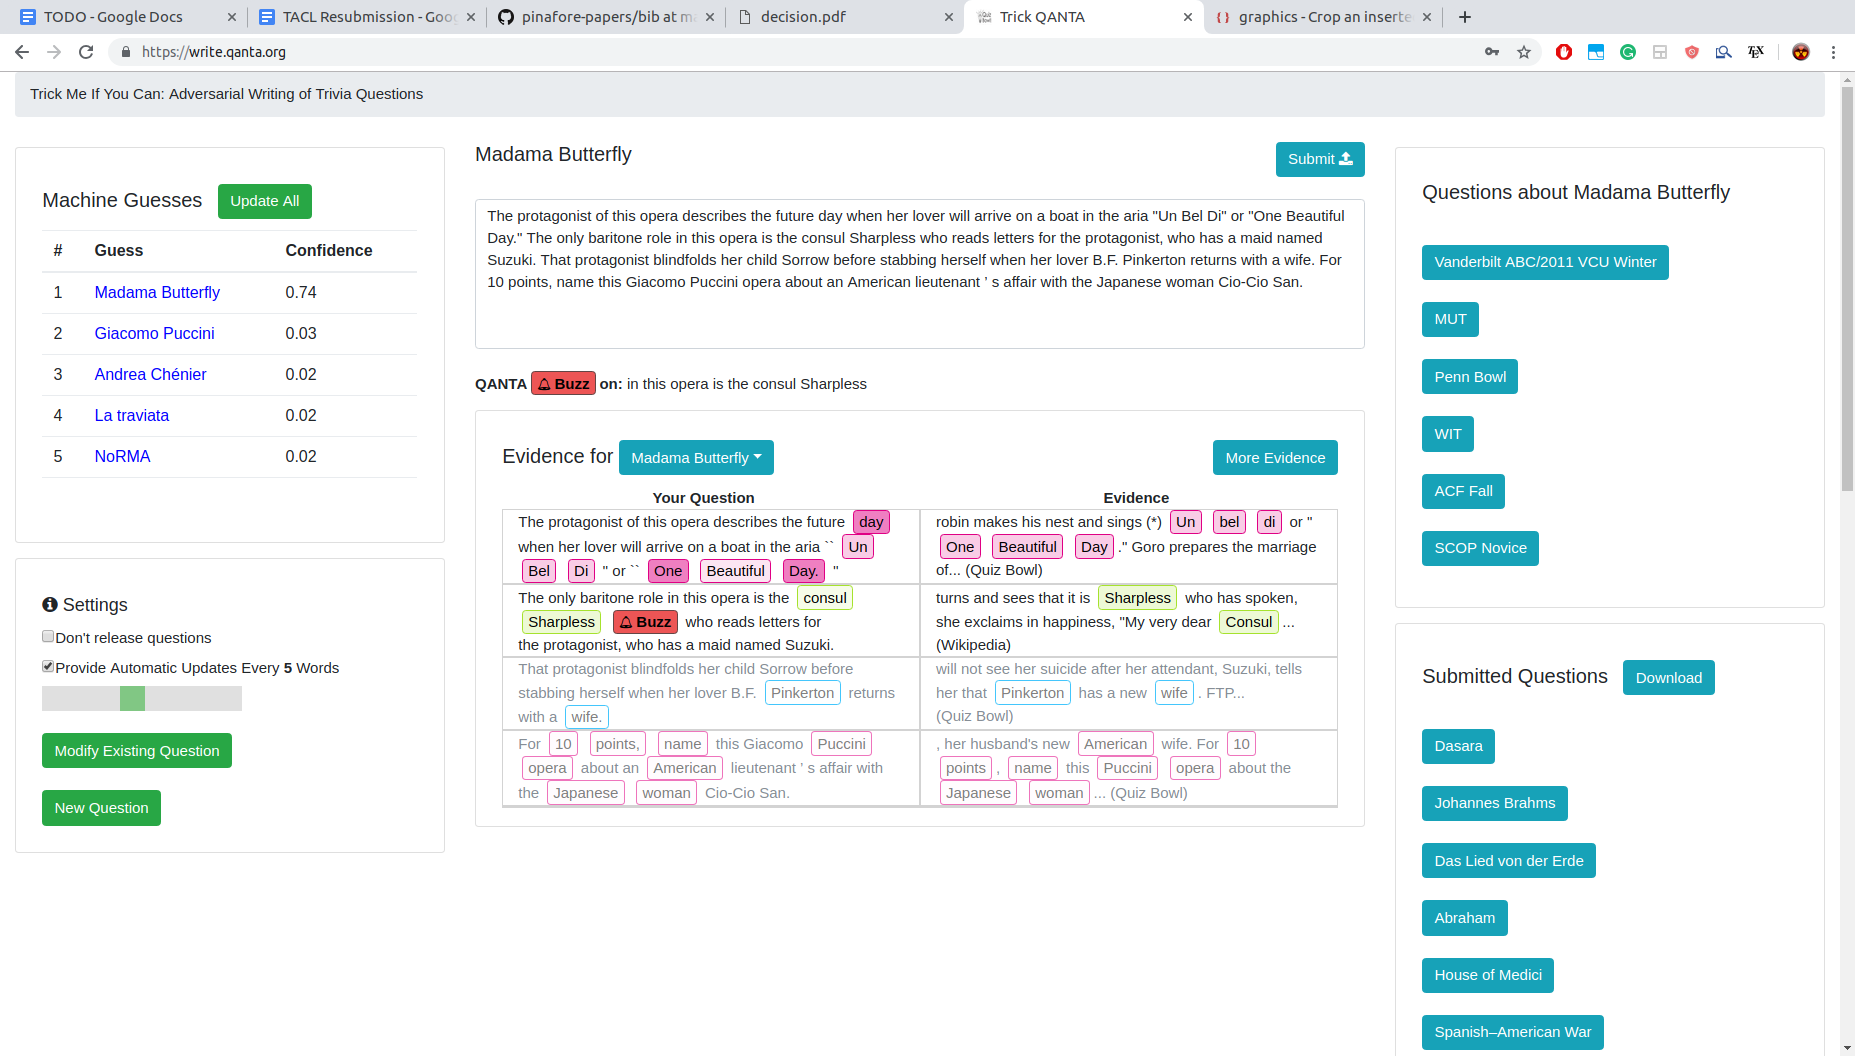
\includegraphics[width=\textwidth, trim={0cm 7cm 16.5cm 5cm},clip]{full_interface}
\caption{The author writes a question (top right), the \abr{qa} system provides
  guesses (left), and explains why it makes those guesses (bottom
  right). The author can then adapt their question to ``trick'' the
  model.}
\label{interface}
\end{figure*}

The authors interact with either the \abr{ir} or \abr{rnn} model through
a user interface\footnote{\url{https://github.com/Eric-Wallace/trickme-interface/}}
(Figure~\ref{interface}). An author writes their question in the upper
right while the model's top five predictions (\textit{Machine
  Guesses}) appear in the upper left. If the top prediction is the
right answer, the interface indicates where in the question
the model is first correct. The goal is to cause the model to
be incorrect or to delay the correct answer position as much as
possible.\footnote{The authors want normal \qb{} questions 
which humans can easily answer by the very end. For popular answers,
  (e.g., \underline{Australia} or \underline{Suez Canal}), writing novel
  final give-away clues is difficult. We thus expect models to often answer correctly
  by the very end of the question.} The words of the
current question are highlighted using the applicable interpretation
method in the lower right (\emph{Evidence}). We do not enforce
time restrictions or require questions to be adversarial: if the
author fails to break the system, they are free to ``give up'' and
submit any question.

The interface continually updates as the author writes.
We track the question edit history to identify recurring model
failures (Section~\ref{sec:limitations}) and understand how
interpretations guide the authors (Section~\ref{sec:help}).

\subsection{Question Authors}

We focus on members of the \qb{} community: they have deep trivia knowledge and craft
questions for \qb{} tournaments~\cite{jennings-06}. We award prizes for questions
read at live human--computer matches (Section~\ref{subsec:live}).

The question authors are familiar with the standard format of \qb{}
questions~\cite{lujan2003writing}. The questions follow a common
paragraph structure, are well edited for grammar, and finish with a
simple ``give-away'' clue. These constraints benefit the adversarial
writing process as it is very clear what constitutes a difficult but
valid question. Thus, our examples go beyond surface level ``breaks''
such as character noise~\cite{belinkov2018synthetic} or syntax
changes~\cite{iyyerscpn2018}. Rather, questions are difficult because
of their semantic content (examples in Section~\ref{sec:limitations}).

\subsection{How an Author Writes a Question}

\AtBeginEnvironment{quote}{\vspace{0.05\baselineskip}}% Stuff before {quote}
\AtEndEnvironment{quote}{\vspace{0.05\baselineskip}}% Stuff after {quote}
To see how an author might write a question with the interface, we walk
through an example of writing a question's first sentence. The
author first selects the answer to their question from the training
set---\underline{Johannes
Brahms}---and begins:
\begin{quote} Karl Ferdinand Pohl showed this composer some pieces on which
  this composer's Variations on a Theme by Haydn were based. \end{quote}
The \abr{qa} system \emph{buzzes} (i.e., it has enough information to
interrupt and answer correctly) after 
``composer''. The author sees that the name ``Karl
Ferdinand Pohl'' appears in Brahms' Wikipedia page and avoids
 that specific phrase, describing Pohl's
position instead of naming him directly:
\begin{quote} This composer was given a theme called ``Chorale St. Antoni'' by the
  archivist of the Vienna Musikverein, which could have been written
  by Ignaz Pleyel.\end{quote}
This rewrite adds in some additional information (there is a scholarly
disagreement over who wrote the theme and its name), and the \abr{qa} system now incorrectly thinks the answer is
\underline{Fr\'ed\'eric Chopin}.
The user can continue to build on the theme, writing \begin{quote}
   While summering in Tutzing, this composer turned that theme into
   ``Variations on a Theme by Haydn''.  \end{quote}
 Again, the author then sees that the system buzzes ``Variations on a
 Theme'' with the correct answer.  However, the author can rewrite it
 in its original German, ``Variationen \"uber ein Thema von Haydn'' to
 fool the system.
 The author continues to
create entire questions the model cannot solve.
